% =============================================================
%  Transmission limits — thermal, voltage drop, angular stability
%  Figures in fig/, copied from presentation/design/ac-transmission/fig/
%  (tl_*.pdf, np_loadability.pdf), generated by that folder's
%  transmission_limits_figures.py and natural_power_figures.py from
%  the exact two-port equations.
% =============================================================
\subsection{Transmission Limits}
\label{sec:limits}

The representation of Section~\ref{sec:ac-transmission} says what a line
does, not what it may be asked to do. Three criteria bound the transfer, and
which of them binds depends almost entirely on length.

\subsubsection{The three criteria}
\label{sec:limits-three}

\paragraph{Thermal.} The conductor temperature sets a current, and with it a
transfer that is independent of length:
\begin{equation}
  P_{th} = \sqrt{3} \cdot U_n \cdot I_{th}
  \label{eq:lim-thermal}
\end{equation}
The limiting mechanism is annealing of the aluminium and, more often, loss
of ground clearance through sag. It is the only one of the three that is a
property of the equipment rather than of the system, and it is weather- and
time-dependent, which is what dynamic line rating exploits.

\paragraph{Voltage drop.} The receiving-end voltage has to stay inside its
band under load. Written on the two-port,
\begin{equation}
  U_S = \left|\underline{A} \cdot \underline{U}_R
             + \underline{B} \cdot \underline{I}_R\right|
      \le 1.0\,\text{p.u.}
  \quad\text{with}\quad
  U_R \ge 0.95\,\text{p.u.}
  \label{eq:lim-voltage}
\end{equation}
Beyond natural loading the line is a net consumer of reactive power, and the
drop grows faster than the transfer. Shunt compensation at the receiving end
raises this limit at the cost of a weaker voltage-stability margin.

\paragraph{Steady-state stability.} The transmission angle must stay far
enough below the crest of the power-angle curve that the system survives the
loss of a parallel element. With a midpoint series bank of degree $k$ the
lossless form is
\begin{equation}
  P_{stab} \approx \frac{U^2}{\left(1-k\right) \cdot X_L}
            \cdot \sin\delta_{max}
  \label{eq:lim-stability}
\end{equation}
and a criterion of $\delta_{max} = 30^\circ$ leaves a factor two on the
lossless maximum. Section~\ref{sec:angular-stability} treats this limit
properly, including why the usable value is well below $P_{max}$.

The loadability of the line is the minimum of the three. Plotted against
length it is the St.~Clair curve.

\subsubsection{Loadability of the reference line}
\label{sec:limits-loadability}

Figure~\ref{fig:tl-loadability} evaluates the three criteria on the 500\,kV
reference line of Section~\ref{sec:reference-line} with the exact two-port
relations, for two boundary conditions. In case~(a) the load sits at the
receiving end with no reactive support, which is the classical St.~Clair
configuration. In case~(b) the line runs between two stiff systems with both
terminals held at 1.0\,p.u., which removes the voltage criterion entirely.
The thermal limit is $I_{th} = 3 \times 1300$\,A at 75\,$^\circ$C, giving
$P_{th} = 3377$\,MW against $P_{nat} = 939$\,MW.

\begin{figure}[!ht]
  \centering
  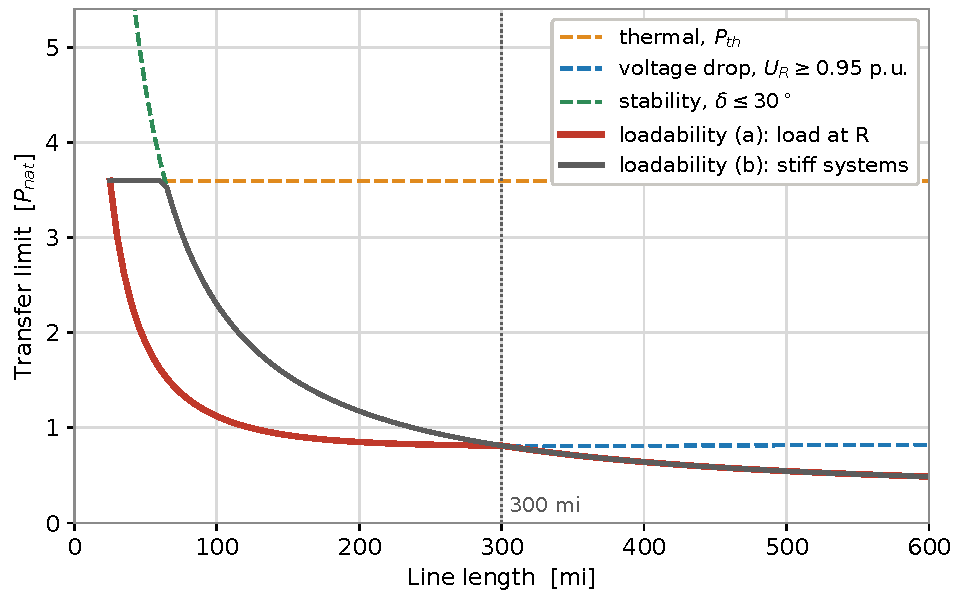
\includegraphics[width=0.78\linewidth]{ac-transmission/fig/tl_loadability.pdf}
  \caption{Loadability of the 500\,kV reference line against length, cases
           (a) and (b), uncompensated}
  \label{fig:tl-loadability}
\end{figure}

In case~(a) the thermal limit binds only to about 25\,mi, after which
voltage drop takes over, and the loadability falls through $1 \cdot P_{nat}$
at 125\,mi. In case~(b) the thermal limit holds to about 60\,mi and angular
stability binds beyond it, with the crossing at 240\,mi. At the 300\,mi
design length both cases give 763\,MW, or $0.81 \cdot P_{nat}$ --- the
voltage and the angle criterion happen to coincide there, and the line
cannot carry even its natural power without compensation.

The boundary condition is not a detail. Holding the receiving end at
1.0\,p.u.\ moves the $1 \cdot P_{nat}$ crossing by 115\,mi on this line. Any
loadability figure has to be quoted with the reactive support it assumes.

\subsubsection{Loadability of the 400\,kV line}
\label{sec:limits-400}

Figure~\ref{fig:np-loadability} repeats the exercise on the 400\,kV, 50\,Hz
line of Section~\ref{sec:natural-power}, with criteria $I \le 2.0$\,kA,
$U_R \ge 0.95$\,p.u.\ and $\vartheta \le 30^\circ$. In case~(a) the thermal
limit holds to 80\,km at $2.3 \ldots 2.4 \cdot P_{nat}$, voltage drop binds
from 120 to 400\,km, angular stability beyond 500\,km, and the curve falls
through $1 \cdot P_{nat}$ at 382\,km. In case~(b) the thermal limit holds to
160\,km, stability binds beyond 200\,km, and the crossing moves to 472\,km.

\begin{figure}[!ht]
  \centering
  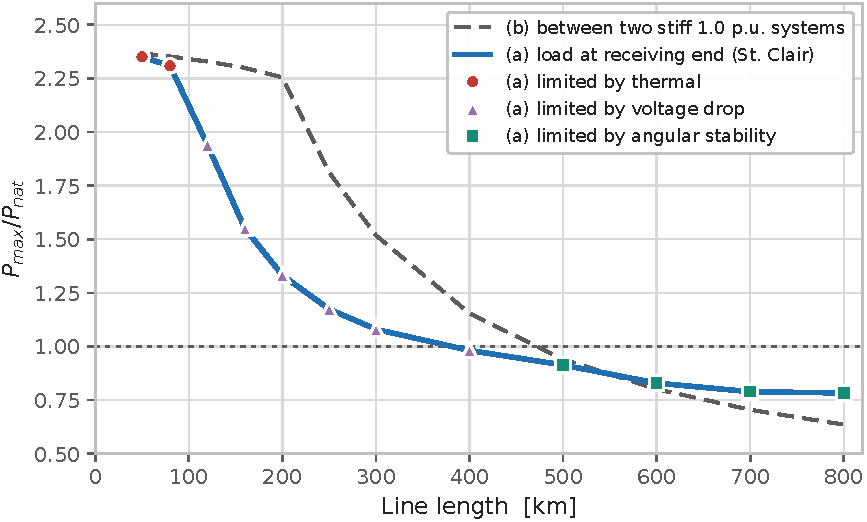
\includegraphics[width=0.78\linewidth]{ac-transmission/fig/np_loadability.pdf}
  \caption{Loadability of the 400\,kV line against length, with $P_{nat}$
           marked}
  \label{fig:np-loadability}
\end{figure}

The shape is the same on both lines: a thermal plateau of about $2 \ldots
2.5 \cdot P_{nat}$ over the first tens of kilometres, then a decay that
crosses natural power somewhere between a quarter and a half of a thousand
kilometres. That is the general statement the St.~Clair curve makes.

\FloatBarrier

\subsubsection{Effect of series compensation}
\label{sec:limits-compensation}

Figure~\ref{fig:tl-loadability-k} repeats case~(b) for a midpoint series
bank of degree $k$, and Table~\ref{tab:tl-k} gives the values at the 300\,mi
design length.

\begin{figure}[!ht]
  \centering
  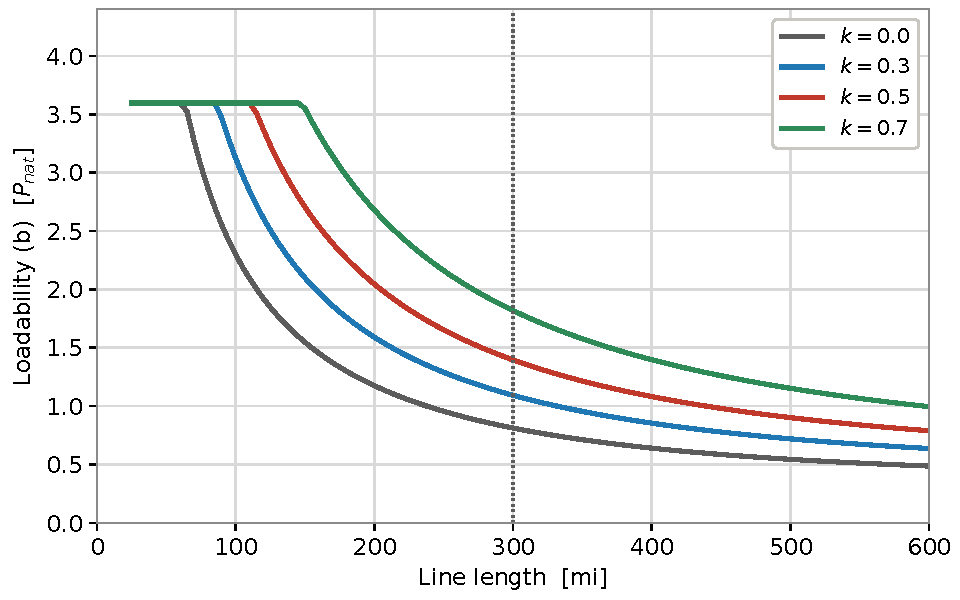
\includegraphics[width=0.74\linewidth]{ac-transmission/fig/tl_loadability_k.pdf}
  \caption{Case (b) loadability of the reference line with a midpoint series
           bank of degree $k$}
  \label{fig:tl-loadability-k}
\end{figure}

\begin{table}[!ht]
  \centering
  \begin{tabular}{@{}c r r r r@{}}
    \toprule
    \textbf{$k$} & \multicolumn{1}{c}{\textbf{$P_{stab}$}}
      & \multicolumn{1}{c}{\textbf{$P_U$}}
      & \multicolumn{1}{c}{\textbf{case (b)}}
      & \multicolumn{1}{c}{\textbf{thermal to}} \\
    & \multicolumn{1}{c}{MW} & \multicolumn{1}{c}{MW}
      & \multicolumn{1}{c}{$P_{nat}$} & \multicolumn{1}{c}{mi} \\
    \midrule
    0   &  763 & 763 & 0.81 &  60 \\
    0.3 & 1027 & 826 & 1.09 &  85 \\
    0.5 & 1311 & 844 & 1.40 & 110 \\
    0.7 & 1708 & 796 & 1.82 & 145 \\
    \bottomrule
  \end{tabular}
  \caption{Effect of a midpoint series bank at 300\,mi on the reference line}
  \label{tab:tl-k}
\end{table}

The bank acts on the stability limit: $k = 0.5$ lifts the 300\,mi
loadability of case~(b) from 0.81 to $1.40 \cdot P_{nat}$. The voltage limit
of case~(a) barely moves, because the $I \cdot X_C$ rise across the bank is
in quadrature with a unity-power-factor load. Series compensation therefore
does not remove the need for reactive support at the receiving end; it
addresses a different limit.

\subsubsection{Equipment limits}
\label{sec:limits-equipment}

The conductor is not always the first thing to run out. Currents follow from
the line-to-line voltage,
\begin{equation}
  I = \frac{S}{\sqrt{3} \cdot U_{LL}}
  \label{eq:lim-current}
\end{equation}
and the switchgear in series with the line carries the same current. The
largest continuous rating available in transmission circuit breakers is
about 5000\,A (Hitachi Energy, GE), so on a high-current scheme the breaker
rating, not the conductor, can set the maximum current and force either a
higher voltage or a second circuit.

\FloatBarrier
